\documentclass[norsk, 10pt,twocolumn]{article}
\usepackage{babel}          % Ordelingsregler, osv
\usepackage[utf8]{inputenc}
\usepackage[T1]{fontenc}
\usepackage{booktabs}       % Ordentlige tabeller
\usepackage{url}            % Skrive url-er
\usepackage{textcomp}       % Den greske bokstaven micro i text-mode
\usepackage{units}          % Skrive enheter riktig
\usepackage{float}          % Figurer dukker opp der du ber om
\usepackage{lipsum}         % Blindtekst
\usepackage{amsmath, amsfonts, amssymb, amsthm}
\usepackage{caption,subfigure,listings, booktabs}
\usepackage{tikz,graphicx}
\usepackage{sectsty}

% Setter fonter
\usepackage{bbold,gillius}
\allsectionsfont{\sffamily} % Sans serif på alle overskrifter
%\renewcommand{\abstractname}{Executive Summary}
\captionsetup{width=.8\textwidth, textfont={small,it},labelfont={small,sf}}
\usepackage[sc,osf]{mathpazo} % Palatino


% Kodelisting
\usepackage{verbatim}
\lstset{language=matlab,breaklines=true,numbers=left} % For hele programmer.
%\lstinputlisting[language=matlab]{fil.m}

% Layout
%\usepackage[top=1.2in, bottom=1.7in, left=1.7in, right=1.7in]{geometry}
\usepackage[top=1.2in, bottom=1.7in, left=.7in, right=.7in]{geometry}
\frenchspacing % Rett mellomrom etter punktum.
\linespread{1.1} % Linjeavstand.
\usepackage[colorlinks=true]{hyperref} % Farge på lenker.

% Egendefinerte kommandoer
\newcommand{\dt}{\, {\rm d}t\, }
\newcommand{\dx}{\, {\rm d}x\, }
\newcommand{\dv}{\, {\rm d}v\, }
\newcommand{\dr}{\, {\rm d}r\, }
\newcommand{\dd}{\, {\text d} }
%\newcommand{\dp}{\ {\rm d}p\ }
\newcommand{\R}{\mathbb{R}}
\def\mean#1{\left\langle #1 \right\rangle}
\renewcommand{\exp}{\mathit{e}}
%\DeclareMathOperator{\dt}{dt}
\newcommand{\mb}[1]{\mathbf{#1}}
\def\para#1{\left( #1 \right)}
\newcommand{\ket}[1]{\left|#1\right\rangle}
\newcommand{\bra}[1]{\left\langle#1\right|}

%, trim = 1cm 7cm 1cm 7cm % PDF-filer som bilde

\begin{document}

% Forside
\begin{titlepage}
\begin{center}

\textsf{\Large FYS4150 - Computational Physics\\[0.5cm]
\rule{\linewidth}{0.5mm} \\[0.4cm]
{ \huge \bfseries  PROSJEKT 2}\\[0.10cm]
\rule{\linewidth}{0.5mm} \\[1.5cm]
{\Large Å løse Schrödingers likning for étt og to elektroner}}\\[1.5cm]
\textsc{}\\[1.5cm]

% Av hvem?

\textsf{\begin{minipage}{0.49\textwidth}
    \begin{center} \large
        Jon Vegard Sparre\\ \url{jonvsp@uio.no} \\[0.8cm]
    \end{center}
\end{minipage}}
%\begin{minipage}{0.49\textwidth}
%    \begin{center} \large
%        Anne-Marthe Hovda\\ \url{annemmho@uio.no} \\[0.8cm]
%    \end{center}
%\end{minipage}}


\vfill

% Dato nederst
\textsf{\large{Dato: \today}}

\end{center}
\end{titlepage}

\abstract{I dette prosjektet ser vi på numerisk integrasjon på tre (fire) måter. Vi starter med Gaussisk kvadratur (GK) i form av Gauss-Legendre og Gauss-Laguerre kombinert med Gauss-Legendre, deretter ser vi på rett fram-Monte Carlo og en litt forbedra Monte Carlo-metode.}

Lenke til Jon Vegards GitHub-domene: \url{https://github.com/jonvegards/FYS4150}

\section*{Introduksjon}
Numerisk integrasjon kan gjøres på mange måter, vi ser her nærmere på metoder som baserer seg på Gaussisk kvadratur og Monte Carlo-teknikker. Førstnevnte er den eldste metoden og ble utviklet før datamaskiner fantes, mens sistnevnte er en litt nyere metode som kom i første halvdel av 1900-tallet. Integralet som vi skal teste disse metodene på er,
\begin{equation}
	\mean{ \frac{1}{|\mb r_1 - \mb r_2|}} = \int\limits_{-\infty}^\infty \dd\mb r_1\dd\mb r_2\, e^{-2\alpha(r_1+r_2)} \frac{1}{|\mb r_1 - \mb r_2|}. \label{integral}
\end{equation}
Dette integralet har en analytisk løsning som er $5\pi^2/16^2$, så vi kan lett sjekke om de numeriske resultatene stemmer.

Gaussisk kvadratur er en integrasjonsmetode som baserer seg på å summere opp funksjonsverdier ganget med en vektfunksjon som vekter leddene i summen forskjellig. De forskjellige vektene blir bestemt av ortogonale polynomer som Legendre- eller Laguerre-polynomer. Vi ser nærmere på utledninga av dette i Teori-delen.

Monte Carlo-metoder baserer også seg på summasjon av funksjonsverdier.

\section*{Teori}
For å skjønne hvordan integrasjonsmetodene virker så kan det lønne seg å se litt på utledninga av de. Som nevnt i introduksjonen så baserer GK seg på summasjon av funksjonsverdier som er vektet forskjellig. I metoder som Simpsons metode så vektes alle integrasjonspunkt likt, og det er ikke alltid like fornuftig. Hvis integranden vår ikke varierer mye over et større intervall, så vil metoder som den ovennevnte konvergere sakte og sørge for at vi bruker unødig mye regnekraft.

Vi kan derfor introdusere GK som kort og godt skrives,
\begin{equation}
	I = \int\limits_{a}^b f(x) \dx \approx \sum\limits_{i=1}^N \omega_i f(x_i).
\end{equation}
Hvor vi da har $\omega_i$ som vektene og $x_i$ er integrasjonspunktene. Det er flere måter å velge vektene på, i dette prosjektet ser vi først på Gauss-Legendre. Den bruker ortogonale polynomer i intervallet $x\in[-1,1]$ med vektfunksjonen $W(x) = 1$. Men for å komme dit må vi først se litt på hvilken rolle vektfunksjonen har. Det viser seg at et integrand som ikke er glatt i integrasjonsintervallet kan gjøres glatt ved å dra ut en vektfunksjon fra den, vi får,
\begin{align}
	I = \int\limits_{a}^b f(x) \dx = \int\limits_{a}^b W(x)g(x) \dx \approx \sum\limits_{i=1}^N \omega_i g(x_i). \label{kvadratur}
\end{align}
Denne vektfunksjonen må  være positiv i hele integrasjonsintervallet slik at $\int_a^b |x|^n W(x)\dx$ er integrerbar. Likn. (\ref{kvadratur}) kalles en GK hvis den kan integrere alle polynomer $p$ eksakt,
$$ 	I = \int\limits_{a}^b W(x)p(x) \dx = \sum\limits_{i=1}^N \omega_i p(x_i). $$
Vi får av dette $2N$ likninger, $N$ for integreringspunktene og $N$ for vektene, dette impliserer at vi kan tilnærme integranden vår $f(x) \approx P_{2N-1}(x)$, en dobling fra metoder som for eksempel Simpons metode. Men hvordan ser polynomet vi tilnærmer integranden med, ut? Vi definerer det til å være,
\begin{equation}
	P_{2N-1} (x) = L_N(x)P_{N-1}(x) + Q_{N-1}(x),
\end{equation}
hvor $L_N(x)$ er Legendre-polynomer av $N$-grad, og $P_{N-1}(x)$ og $Q_{N-1}(x)$ er polynomer av grad $N-1$ eller lavere. Vi forutsetter nå at integrasjonsintervallet er $[-1,1]$ siden Legendrepolynomer er definert i det intervallet, vi må altså huske på å endre variablene våre slik at integrasjonsgrensene passer med intervallet til Legendrepolynomene. Likninga ovenfor kan settes inn i integralet vårt og vi kan bruke ortogonalitetsegenskapene til Legendrepolynomene slik at vi får
\begin{equation}
	\int\limits_{-1}^1 P_{2N-1} (x) \dx = \int\limits_{-1}^1 L_N(x)P_{N-1}(x) + Q_{N-1}(x) \dx = \int\limits_{-1}^1  Q_{N-1}(x) \dx
\end{equation}

\section*{Metode}

\section*{Resultat}

\section*{Numerisk stabilitet og presisjon}

\subsection*{Konklusjon}



\end{document}

%\begin{figure}[H]
%	\centering
%	%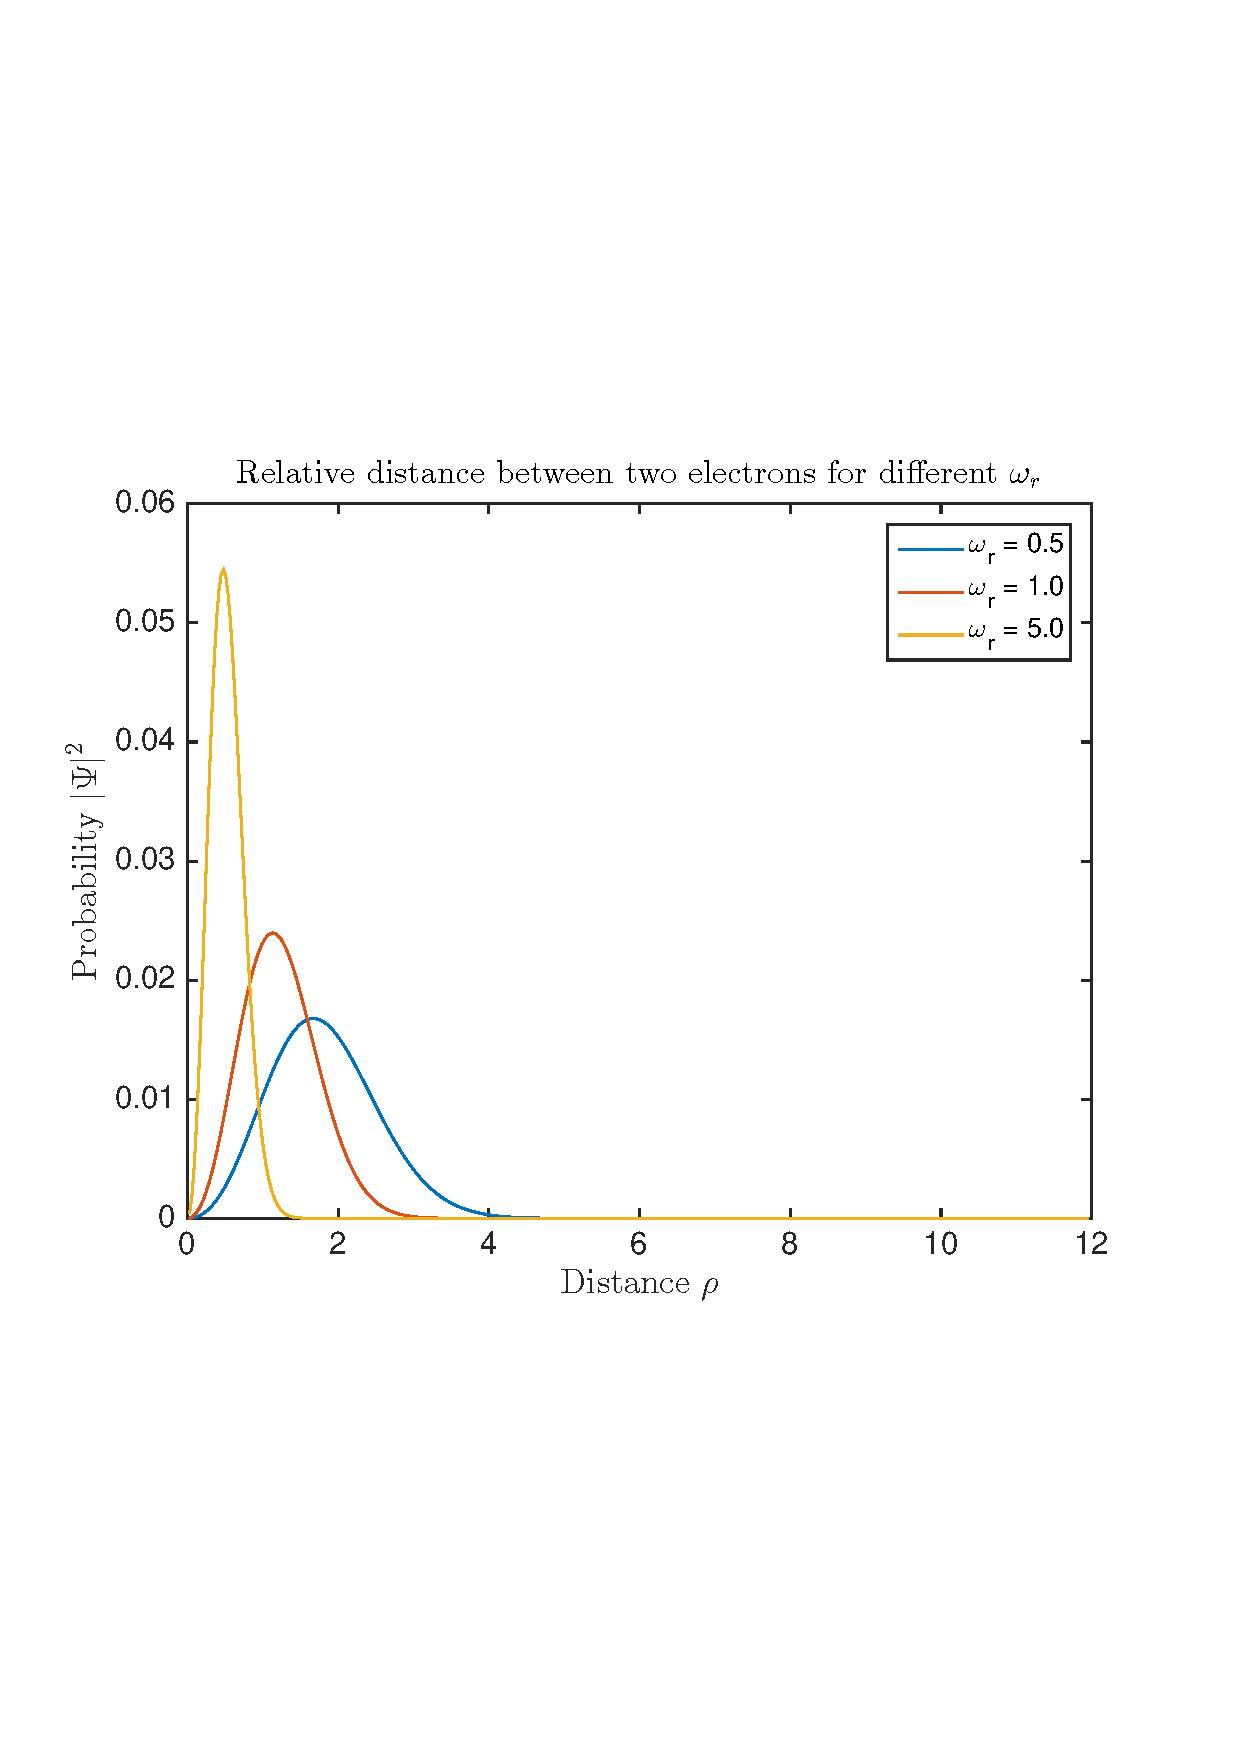
\includegraphics[scale = 0.5, trim = 1cm 7cm 1cm 7cm]{omega_05_1_5.pdf}
%	\caption{Den relative distansen mellom to elektroner for forskjellige verdier av $\omega_r$ ved $n = 400$. Toppunktene til sannsynlighetsfordelingene ligger nærmere null enn da $\omega_r=0.01$, \emph{i.e.} elektronene er nå nærmere hverandre.}
%	\label{fig:n400}
%\end{figure}

%\begin{table}[H]
%  \centering
%  \begin{tabular}{ l l }
%    \toprule
%    $\epsilon$ & $|\Delta\lambda_0|$ \\
%    \midrule
%    $10^{-1}$ & $8.8\cdot10^{-4}$ \\
%    $10^{-2}$ & $4.47\cdot10^{-6}$ \\
%	$10^{-3}$ & $1.63\cdot10^{-7}$ \\
%	$10^{-4}$ & $4.63\cdot10^{-10}$ \\
%	$10^{-5}$ & $1.30\cdot10^{-11}$ \\
%	$10^{-6}$ & $2.57\cdot10^{-13}$ \\
%	$10^{-7}$ & $2.04\cdot10^{-13}$ \\
%	$10^{-8}$ & $2.04\cdot10^{-13}$ \\
%	\bottomrule
%  \end{tabular}
% % \caption{Differanse mellom Armadillos og Jacobis metodes løsning av laveste egenverdi. For $\epsilon < 10^{-7}$ klarer ikke datamaskinen lenger å gi en nøyaktig differanse mellom resultatene siden de er så like. Til tross for at Jacobis metode er en treg metode, så blir den ganske nøyaktig.}
%%  \label{tab:jmarm}
%\end{table}